\documentclass{article}
\usepackage{graphicx,float}
\usepackage{amsmath,latexsym,amsfonts,amssymb,amsthm}

\usepackage[utf8]{inputenc}
\usepackage[english]{babel}
\usepackage[letterpaper,top=2cm,bottom=2cm,left=3cm,right=3cm,marginparwidth=1.75cm]{geometry}
\renewcommand{\baselinestretch}{1.667}


\title{Optimization Methods PS s7 Lab 3}
\author{Joris Plaščinskas}
\date{\today}


\begin{document}


\maketitle
\section*{Short Introduction}
By mistake I implemented the same objective function as in the previous lab (maximizing the volume of a cube with surface plots as input). In order not to redo the whole lab in the end I will derive the x, y and z from the plots.

\section*{2 - Function Values At $X_0$, $X_1$, $X_m$}
\begin{table}[h]
    \centering
    \begin{tabular}{|l|c|c|c|}
        \hline
         & $X_0$ & $X_1$ & $X_m$ \\
        \hline
        $f$ & $-0.0$ & $-0.125$ & $-0.0$ \\
        \hline
        $g_1$ & $-1$ & $2$ & $-0.8$ \\
        \hline
        $h_1, h_2, h_3$ & $0,\ 0,\ 0$ & $-1,\ -1,\ -1$ & $0,\ -0.2,\ 0$ \\
        \hline
    \end{tabular}
    \caption{Function evaluations at points $X_0$, $X_1$, and $X_m$.}
\end{table}


\section*{3 - Code}
\begin{figure}[H]
    \centering
    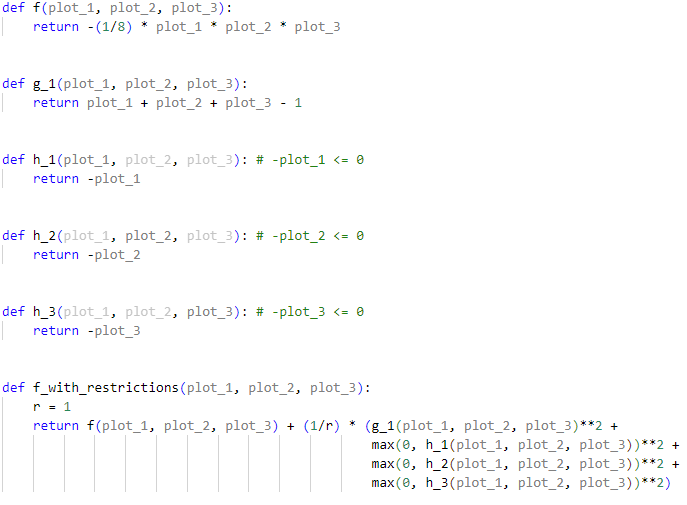
\includegraphics[width=0.8\textwidth]{functions.png}
    \caption{Ojective and Restriction Functions}
    \label{fig:example}
\end{figure}


\section*{4 - Initial r Value Effect On Penalty Values}
\begin{figure}[H]
    \centering
    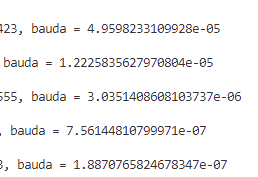
\includegraphics[width=0.3\textwidth]{penalty-1.png}
    \caption{r = 1}
    \label{fig:example}
\end{figure}

\begin{figure}[H]
    \centering
    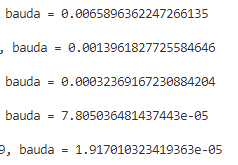
\includegraphics[width=0.3\textwidth]{penalty-10.png}
    \caption{r = 10}
    \label{fig:example}
\end{figure}
These pictures indicate that the lower the initial r value is the lower the penalty function's value will be during training. Which makes sense, because the total penalty is 1/r times the penalty function's value, which means that with higher r values the function parameters can stride away further from the restrictions without receiving much total penalty, leading to the increase of penalty function's value.

\section*{6 - Results}
I got very similar results for all starting X's, each plot was $0.333$... which is $\sim \frac{1}{3}$. However, because the task was not to find the optimal plot values, but rather the optimal x, y and z values. We will derive them using system of equations:

\[
\begin{cases}
2xy = \frac{1}{3} \\
2xz = \frac{1}{3} \\
2yz = \frac{1}{3} \\
\end{cases}
\]

\[
\begin{aligned}
xy = xz \\
y = z \\
xy = yz \\
x = z \\
x = y = z \\
2x^2 = \frac{1}{3} \\
x^2 = \frac{1}{6} \\
x = \pm \frac{1}{\sqrt{6}} \\
\end{aligned}
\]

\[
\begin{cases}
x = \dfrac{1}{\sqrt{6}} \\
y = \dfrac{1}{\sqrt{6}} \\
z = \dfrac{1}{\sqrt{6}} \\
\end{cases}
\]

\[
\begin{cases}
x = -\dfrac{1}{\sqrt{6}} \\
y = -\dfrac{1}{\sqrt{6}} \\
z = -\dfrac{1}{\sqrt{6}} \\
\end{cases}
\]

The negative solution does not satisfy the constraints, so the solution is that the rectangle shaped-box should be of shape: $x = y = z = \dfrac{1}{\sqrt{6}}$.


\end{document}